\chapter{Behaviour analysis of antennas}
In this chapter we analyse and discuss each antenna behaviour, looking at the results obtained in predicting the gain solutions from each experiment of our learning algorithms for both polarization H in Section \ref{Hp} and V polarization in Section \ref{Vp}. 

\section{Pointing sensor distribution}
\begin{figure}[H]
    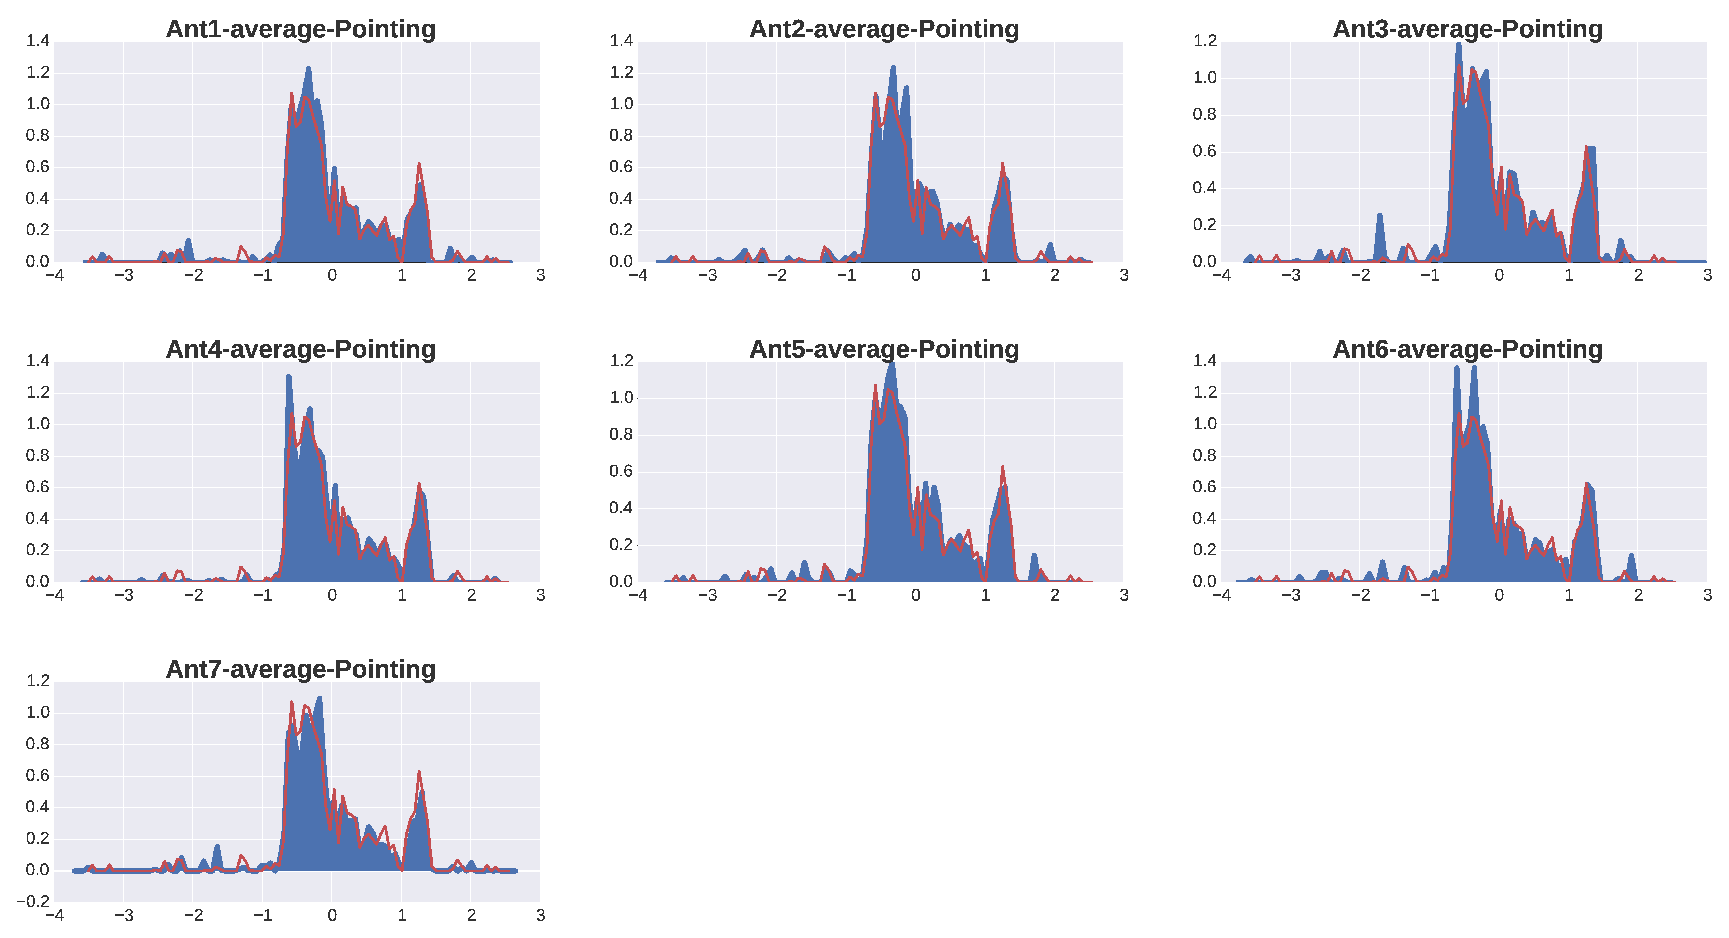
\includegraphics[ height=12cm, width=16cm]{images/Distribution.eps}
    \caption{This figure shows the distribution of the averaged pointing data per antenna during the tracking of the calibrator source PKS1613-586. The blue plot represents the average of all the pointing sensors per antenna, and the red line is the reference probability distribution for all KAT-7 antennas.}
    \label{Point}
\end{figure}
 Figure \ref{Point} illustrates how the pointing sensor data per antenna are distributed. This gives details about whether or not the antennas were pointing at the same position with reference red line as shown in Figure \ref{Point}. One observes that each antenna pointing is distributed differently from the reference probability distribution. These small offsets might have contributed to prediction errors of amplitude and phase gain solutions.

\section{H-polarization amplitude and phase}
\label{Hp}
In this section we show the behaviour of each antenna phase and amplitude for H-polarization  with respect to each model used. We evaluate each antenna behaviour using the RMSE computed during test-time in section \ref{sec3}.   

As seen in Figure \ref{phase}, the gain phase solution obtained from CASA for antenna 5 is zero. This is due to the selection of antenna 5 as a reference antenna during the calibration of $G$ solutions. Fundamentally, the baseline visibility phases measured by interferometry are exclusively different between antennas, and so no absolute phase reference exists \citep{taylor1999synthesis}. Antenna-based calibration solutions thus have phases that are constrained only to satisfy the observed visibility phases; further, each solution in time is formally independent of all others \citep{taylor1999synthesis}, though stability (or at least continuity) in time is expected. Therefore, to assert phase continuity in time, it is conventional practice to assign a reference antenna whose phase will be held constant at zero in time. Also, it is best to choose a reference antenna that never drops out \citep{editioncasa}. 

\begin{figure}[H]
  \centering
    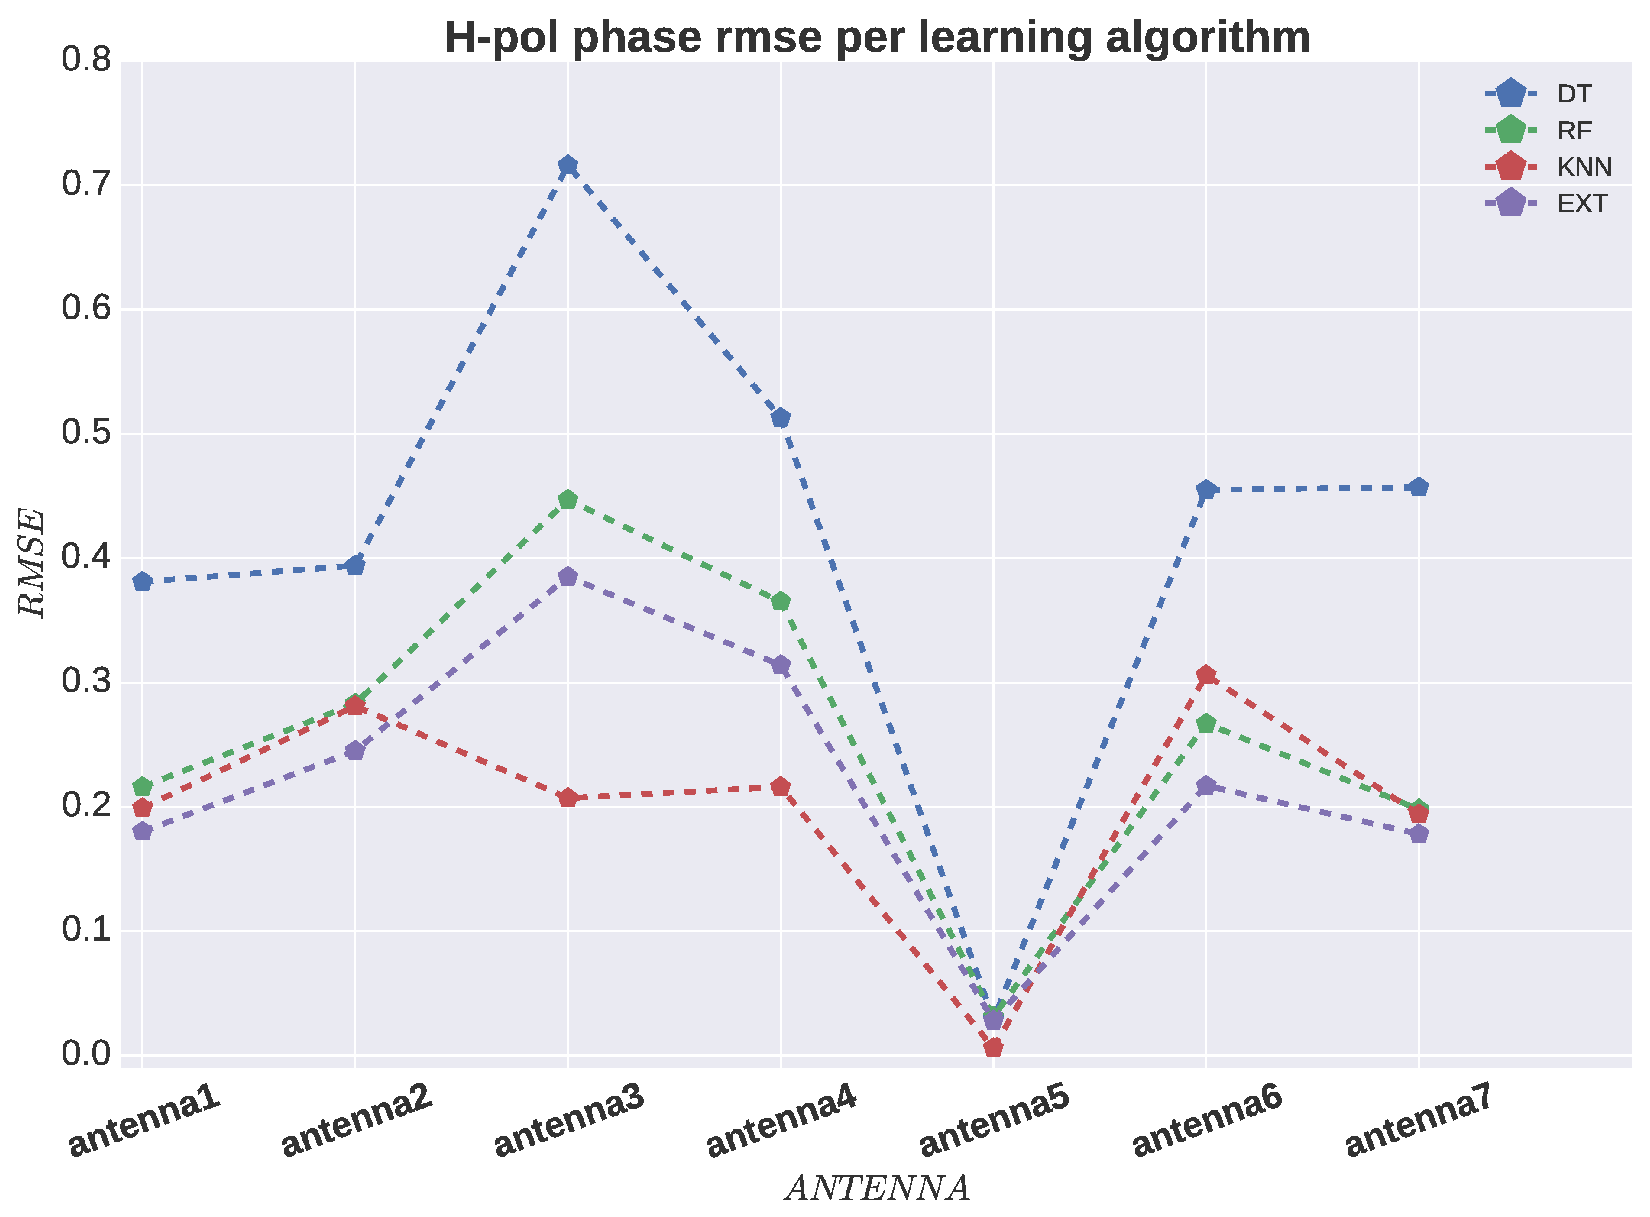
\includegraphics[width=0.6\textwidth]{images/Hpol-phase.eps}
    \caption{Root mean square error for each learning algorithm in predicting the h polarization phase gain solutions for each antenna. The blue, green, red and purple lines represent the different learning algorithms used in the experiment.}
  \label{phrm}
 \end{figure}
From the experiment in Section \ref{sec3} and Figure \ref{phrm}, one observes that the learning algorithms have learned this behaviour pattern with rms error accuracy $\approx$ 0, resulting in predicting zero phase gain solutions for antenna 5. We validated our models looking at three observational validation data sets namely: observation test-1 and observation test-2. We provide our models with sensor data during tracking of the calibrator source PKS1613-586 as input. The phase output predictions in Figures \ref{obs5}, \ref{obs6}, \ref{obs7}, \ref{obs8}, \ref{obs9}, \ref{obs10}, \ref{obs11}, \ref{obs12}  shows that the models have learned to generalize for the reference antenna, by predicting zero phases for antenna 5 H and V polarization as trained, assuming that the antenna was stable without any drop-outs during the period of the observation. In Figure \ref{phrm}, though the models were supposed to perform differently because of their parameter settings, one notices that the random forest, K-nearest neighbor and the extremely randomised trees methods are very close to one another in rms error as a function of antenna 1H, 2H, 5H, 6H and 7H, whereas there are large large rms error bars in each model per antenna 3H and 4H. Such behaviour gives one an idea about the instability of these two antennas. Figure \ref{phrm} also illustrates which model can be used for better predictions of H polarization phase gain solutions. In this case, one observes that the decision tree model has larger rms error scatter than the random forest, K-nearest neighbors and the extremely randomized trees models. As discussed in Chapter 2, though we have used a randomised search algorithm to determine the optimal choice of parameters at each node, decision trees are still prone to over-fitting, especially when a tree is particularly deep, since it gets specific and complicated.Thus this leads to an increase in rms error for the decision tree model, as shown in \ref{phrm}. Such behaviour is referred to as model biasness. Figure \ref{obs5} can be used as one of the examples to show that the decision tree model has not learned to generalize, since it predicts the wild phase solutions when compared to CASA. Thus we introduced the ensemble tree-based and nearest neighbor methods to prevent overfitting. The random forest and extremely randomized tree model in Figures \ref{obs6} and \ref{obs8} predict fairly stable H polarization phase solutions for observation test-1 and test-2 with antenna 6 and 7 close to CASA. As for the K-nearest neighbor algorithm, it performs poorly in predicting the H polarization phase solutions with large scattering and non-constant points over time when feeding it with the validation sets. 
  
One of the causes of this poor prediction could be the small value of K chosen by the randomised search parameter optimisation algorithm. i.e., if the training data set is large but K is too small, then one still runs the risk of overfitting. For example, for K = 3 and a really large data set, there is a reasonable chance that there will be two noisy data points that are close enough to each other to outvote the correct data points in some region. On the other hand, if K is chosen to be too large, then one may end up smoothing things out too much and eliminating some important details in the distribution. 
\begin{figure}[H]
  \centering
    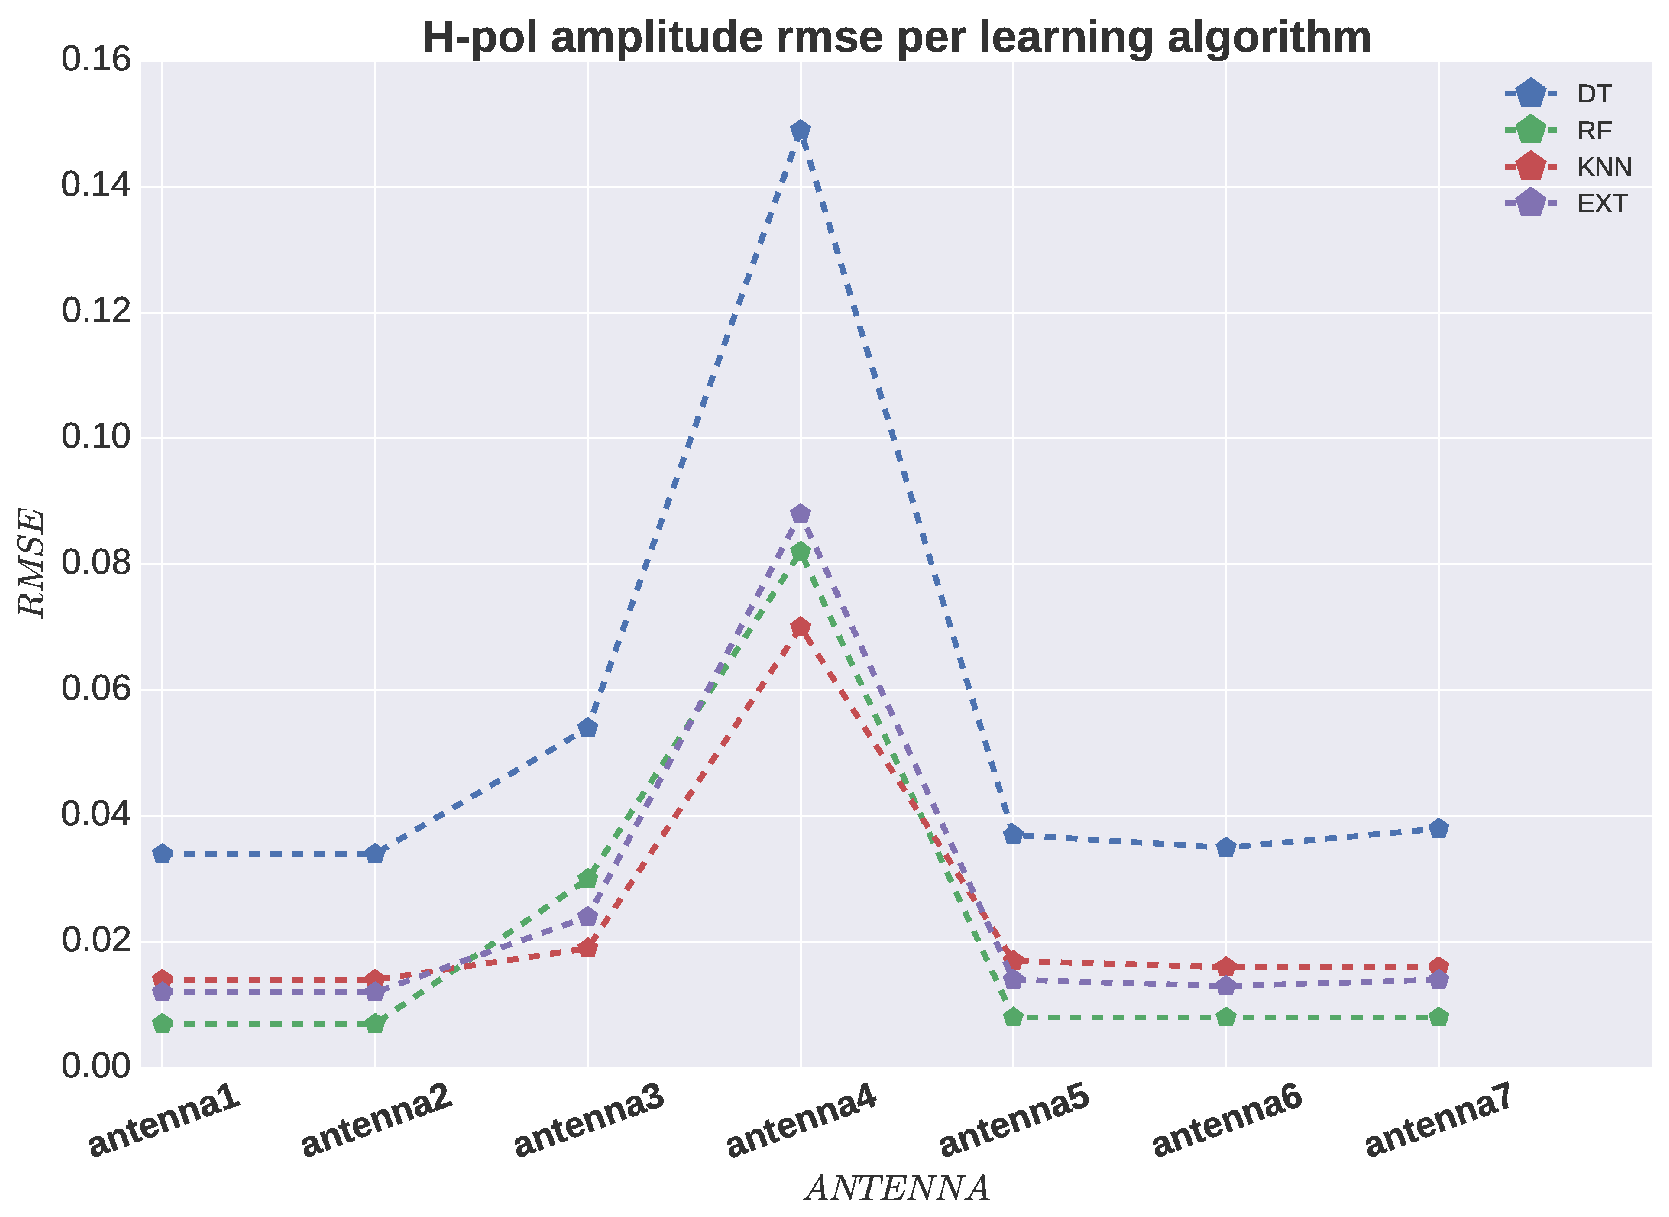
\includegraphics[width=0.6\textwidth]{images/Hpol-amp.eps}
    \caption{Root mean square error for each learning algorithm in predicting the h polarization amplitude gain solutions for each antenna. The blue, green, red and purple lines represent the different learning algorithms used in the experiment.}
  \label{amprm}
 \end{figure} 

From the plot in Figure \ref{amprm}, one observes that the random forest, K-nearest neighbor, and extremely randomized trees learned to predict the H polarization amplitude gain solutions with an rms error accuracy of less than $0.02$, which is much better than the phase prediction in Figure \ref{phrm}. Similar to H polarization phase prediction, one observes a large rms error variation on antenna 3H and 4H in all four models, with decision trees having larger rms error scattering than the rest. From validation data sets, Figures \ref{da2}, \ref{da3} show the decision tree output prediction from all the observation tests, and one observes that the decision tree model cannot generalize well for different new observational sets, thereby producing flat amplitude. However, these models managed to learn the most critical part, i.e., the sinusoidal variation of the gain amplitude solutions over time as shown in Figures \ref{ra2}, \ref{ra3}, \ref{ea2}, \ref{ea3} for the validation dataset. Since the target of the experiment is the calibrator PKS1613-586, which was considered a bright source and a good calibrator during KAT-7 commissioning, we therefore compare the H polarization amplitude experimental solutions with ones obtained from CASA through calibration of the validation data sets. We observe that the machine learning amplitude is lower than CASA with a factor of 33.33$\%$ for observation test-1 and 22.22 $\%$ for observation test-2. On the other hand, the K-nearest neighbor seems to have failed in observation test-1 and predicted reasonably close to CASA for observation test-2 and test-3.

In Figure \ref{ra2} and \ref{ea2}, The model predicts a drop in amplitude as a function of time in the middle of the observation from 0.12 to 0.09 level of CASA, while as the true amplitude have not dropped. From this unique behaviour observed, we can conclude that it is either due to prediction failure as the models have been trained on limited amount of observations and therefore failing on different observation settings, or it could be a behaviour that CASA did not detect as it does not include sensor data when calculating its calibration solutions.
\section{V-polarization amplitude and phase}
\label{Vp}
\begin{figure}[H]
  \centering
    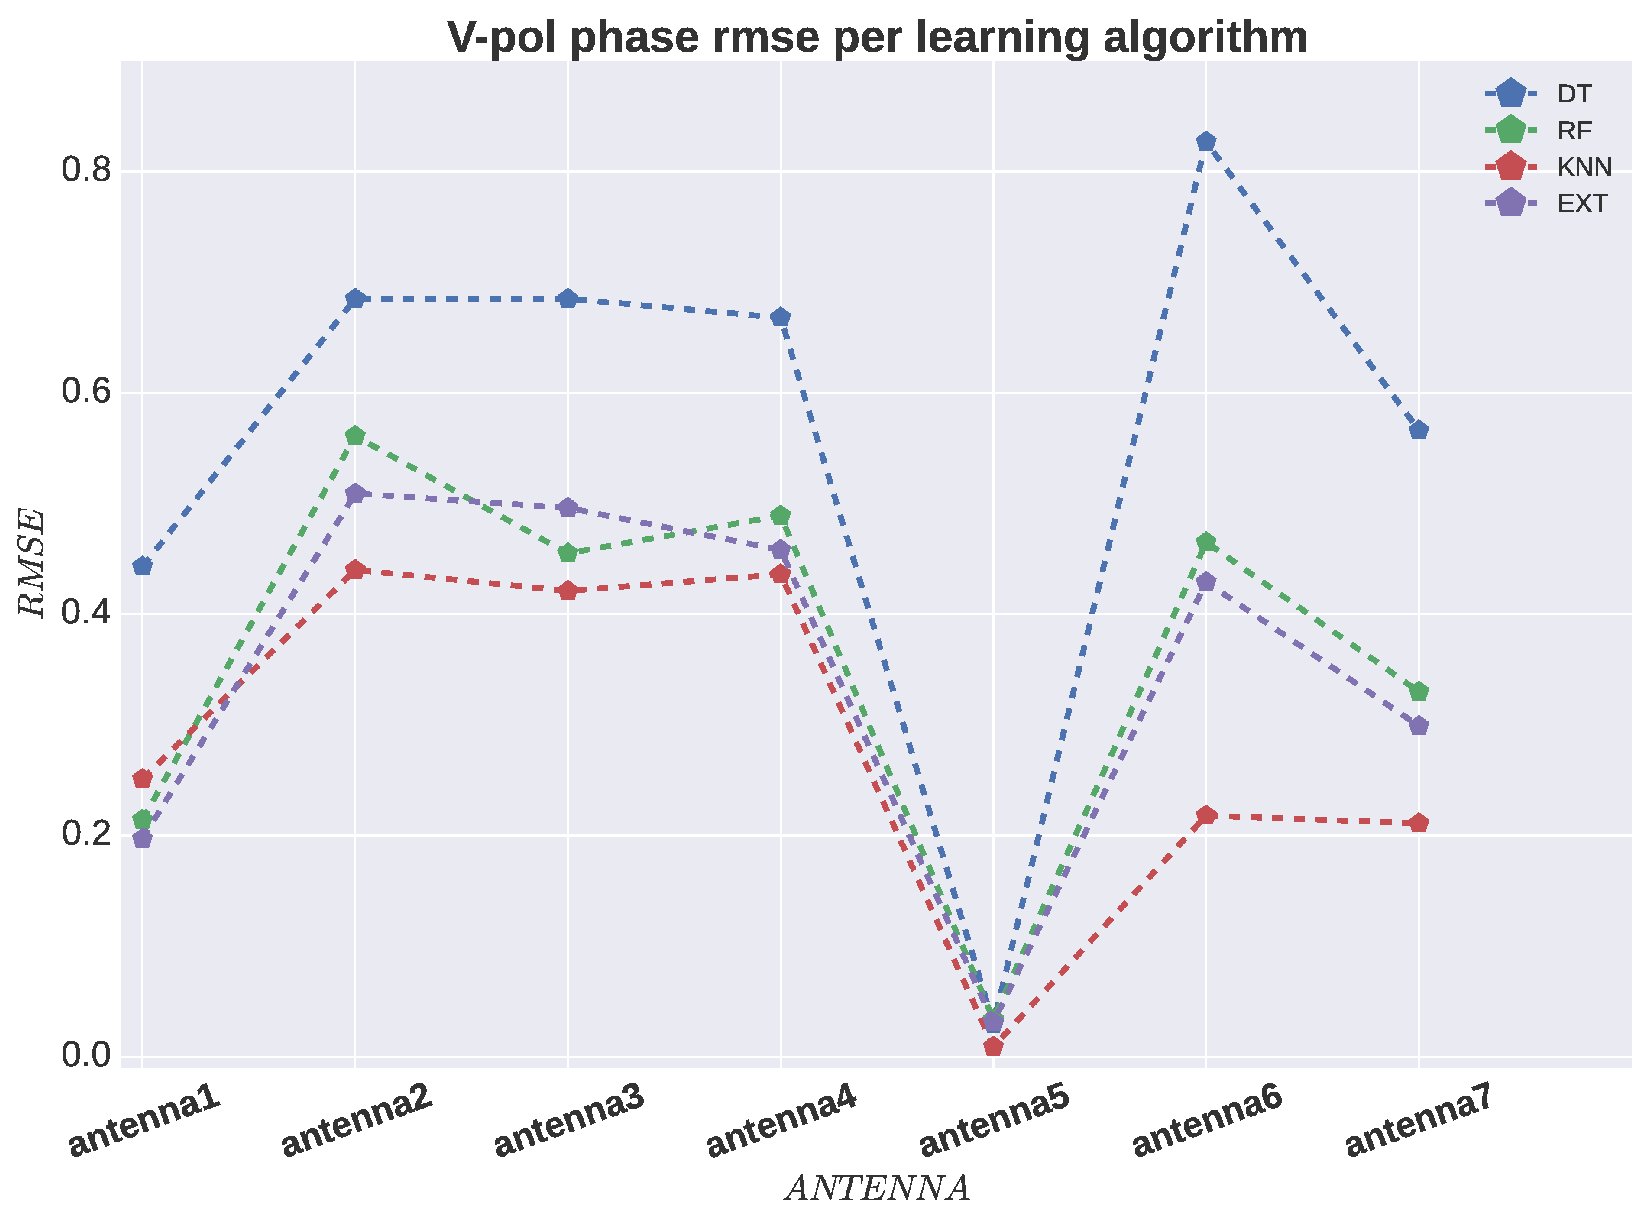
\includegraphics[width=0.6\textwidth]{images/Vpol-phase.eps}
    \caption{Root mean square error for each learning algorithm in predicting the V polarization phase gain solutions for each antenna. The blue, green, red and purple lines represent the different learning algorithms used in the experiment.}
  \label{phrmv}
 \end{figure}
 
The model behaviour for the V polarization phase solutions experiment in Figure \ref{phrmv} is closely similar to Figure \ref{phrm} H polarization in terms of rms error instabilities. We observed large rms error bars in each model per antenna 2V, 6V and 7V and much lower at antenna 1V, 3V, 4V, and 5V for random forest, K-nearest neighbors and the extremely randomized trees models. When feeding the models with the both both validation datasets test-1 and test-2, one observes that the random forest and extremely randomized tree in Figure \ref{obs6} and \ref{obs8} predict fairly stable V polarization phase solutions in antenna 5, antenna 6 for time index < 80, antenna 7 for time index > 80 and fails on antenna 1, 2,3, and 4.

In Figure \ref{phrm} and \ref{phrmv}, we further observe that antennas with rms error > 0.5 $^\circ$ i.e, antenna 2,3,4 have wild phase solution for H and V polarization when predicting on validation dataset as shown in Figure \ref{obs6}, \ref{obs7}, \ref{obs8},\ref{obs10}, \ref{obs11}, \ref{obs12}. 
\begin{figure}[H]
  \centering
    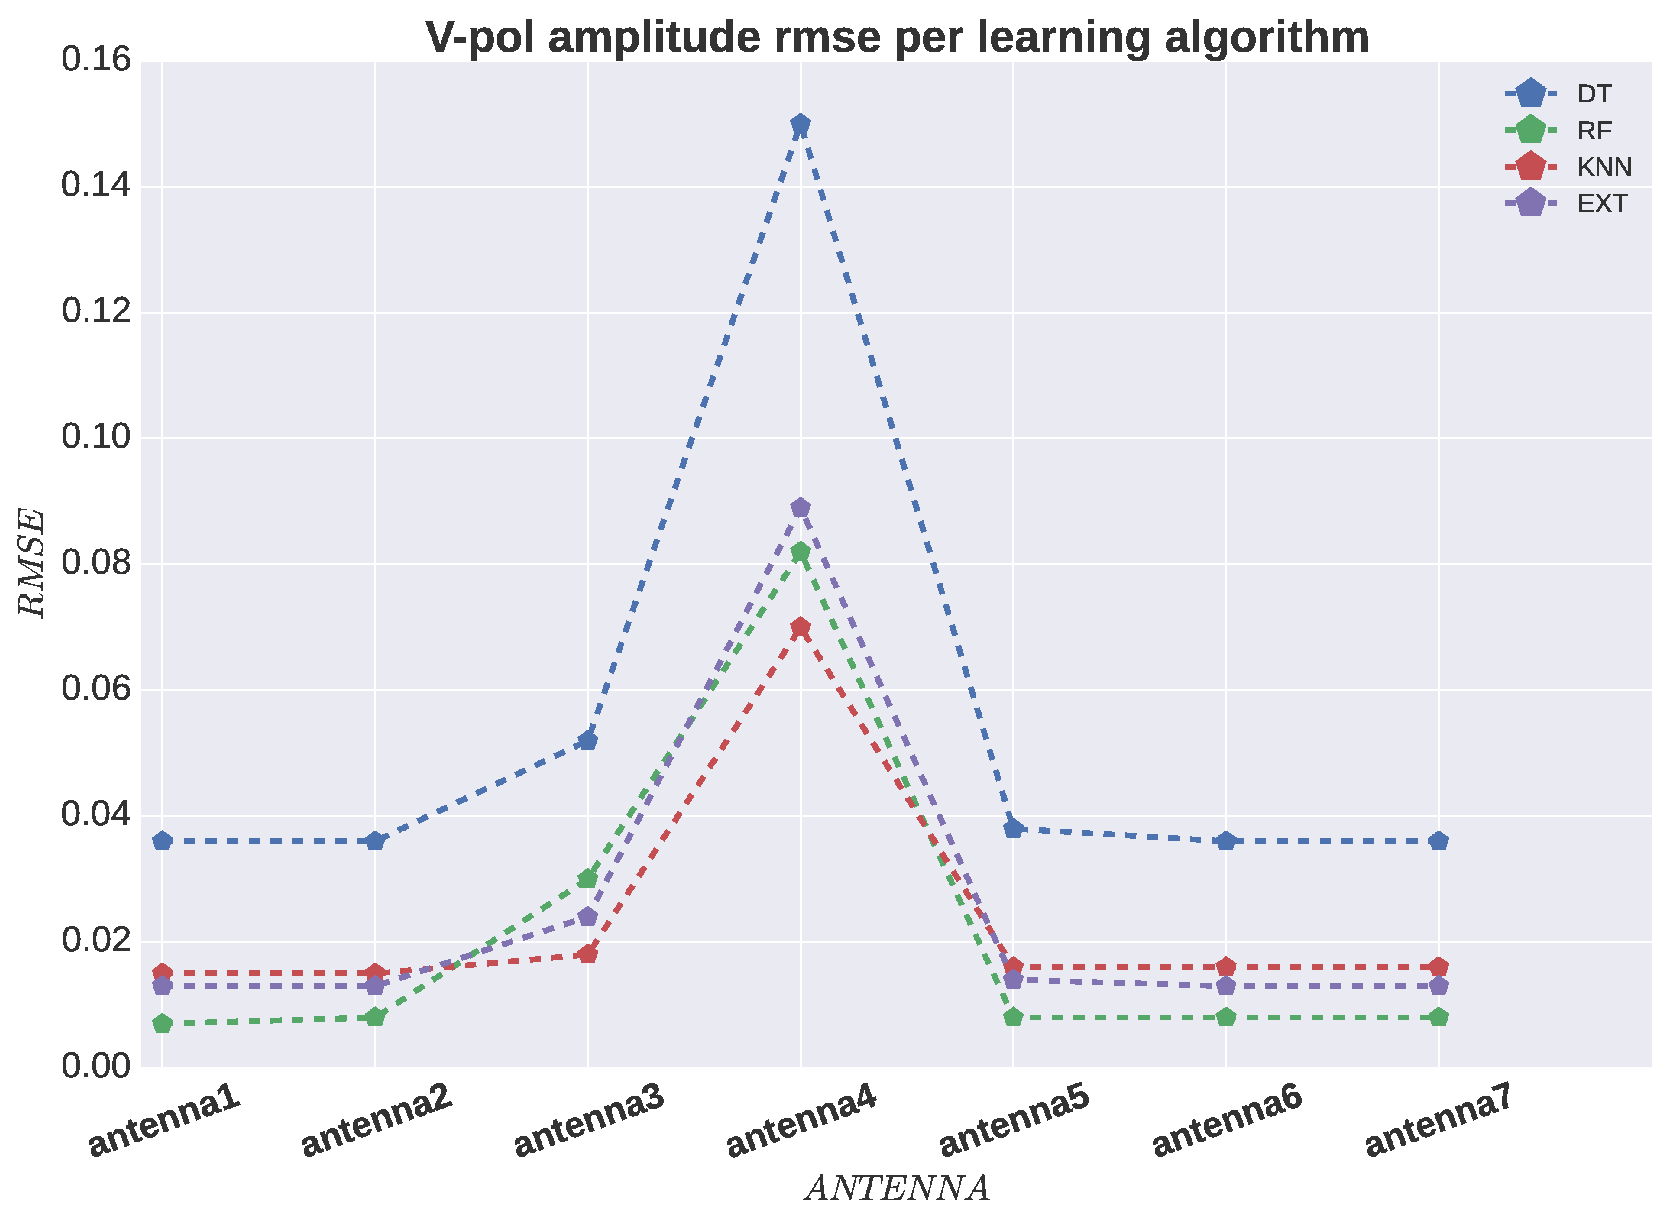
\includegraphics[width=0.6\textwidth]{images/Vpol-amp.eps}
    \caption{Root mean square error for each learning algorithm in predicting the V polarization amplitude gain solutions for each antenna with different colours representing different learning algorithms used in the experiment.}
  \label{amprmv}
 \end{figure} 

The V polarization rms error is no different from H polarizations as shown in Figures \ref{amprm} and \ref{amprmv}, where the rms error in both polarization for all the antennas is measured and rated the same. We observe that the machine learning amplitude is lower than CASA with a factor of 33.33$\%$ for observation test-1 and 22.22 $\%$ for observation test-2. In Figures \ref{amprm} and \ref{amprmv} for H and V polarization, antennas with measured rms error > 0.05, i.e, are showing wild amplitude solutions prediction when feeding the random forest, K-nearest neighbor and extremely randomised models with validation datasets as shown in Figures  \ref{ra2}, \ref{ka2}, \ref{ea2}, \ref{ra3} ,\ref{ka3}, \ref{ea3} for antenna 4. This shows that the model have poorly learned the amplitude solution behaviour of this antenna. From this we can therefore conclude that amplitude solutions with rms error of 0.1 is huge.

From the analysis above, one therefore concludes that the random forest and extremely randomised trees are the better models for predicting the amplitude and phase gain solutions followed by the K-nearest neighbor. However, these models have learned to predict the amplitude gain solutions better than phase. This is most likely due to the fact that the machine learning models were trained on limited amount of data, and therefore cannot fully predict what the sky will be doing, since the phase varies quickly over time as a function of antenna-based (ground) and sky-based effects. As for amplitude, most of its effect are based on instruments and the environment around it, hence it has been doing better than phase prediction in our experiment. Some of the limitations of our experiment may be due to training being done on time-based calibration solutions rather than frequency (bandpass). 

When comparing the bias/variance of the tree-based methods, one observes that algorithm randomization increases bias and variance of individual trees, but  may decrease their variance with respect to the learning sample \citep{geurts2006extremely}. The part of the variance due to randomization can be cancelled out by averaging over a
sufficiently large ensemble of trees. Overall, the bias/variance tradeoff is different in regression than in classification problems;
in particular, classification problems can tolerate high levels of bias of class probability estimates without yielding high classification error rates \citep{geurts2006extremely}. 

During model training, the random forests method does the pre-sorting on the learning sample before growing all trees to avoid having to re-sort it each time a node is split. This pre-sorting reduces the computing times of this method. The implementation of extremely randomized trees, does not use pre-sorting, which is a further advantage when dealing with problems with very large samples, where it may not be possible to keep in memory a sorted copy of the learning sample for each candidate feature. Since pre-sorting requires on the order of $nN\log N$ operations, it makes the
computational complexity of random forests depend linearly on the number of features. Hence, for very large numbers of attributes the computational advantage of extra-trees is even higher \citep{geurts2006extremely}.



%An average research project may contain five chapters, but I didn't plan my work properly
%and then ran out of time. I spent too much time positioning my figures and worrying
%about my preferred typographic style, rather than just using what was provided.
%I wasted days bolding section headings and using double slash line endings, and 
%had to remove them all again. I spent sleepless nights configuring manually numbered lists
%to use the \LaTeX\ environments because I didn't use them from the start or understand
%how to search and replace easily with texmaker.
%
%Everyone has to take some shortcuts
%at some point to meet deadlines. Time did not allow to test model 
%B as well. So I'll skip right ahead and put that under my Future Work section.
%
%
%\section{This is a section} 
%
%Some research projects may have 3, 5 or 6 chapters. This is just an example. 
%More importantly, do you have at close to 30 pages?  
%Luck has nothing to do with it. Use the techniques suggested for
%writing your research project.
%
%Now you're demonstrating pure talent and newly acquired skills. 
%Perhaps some persistence. Definitely some inspiration. What was that about perspiration? 
%Some team work helps, so every now and then why not browse your friends' research project and provide
%some constructive feedback?
%
%\subsection{Subsubsections are disabled}
%
%Vivamus faucibus arcu ut cursus maximus. Aenean ac aliquet nulla. Duis efficitur varius malesuada. Etiam finibus risus et condimentum commodo. Mauris interdum ligula ut lacinia blandit. Curabitur commodo, mauris vel porttitor semper, ante risus pellentesque ipsum, non commodo sapien massa quis tortor. Vestibulum ante ipsum primis in faucibus orci luctus et ultrices posuere cubilia Curae; Phasellus ac massa commodo purus placerat pharetra id ut ex. Nam malesuada, turpis vel iaculis sodales, nisl ante fringilla tellus, et efficitur nisl felis at ligula. 
